On choisit au hasard, sans regarder, une des figures suivantes :
\begin{center}
    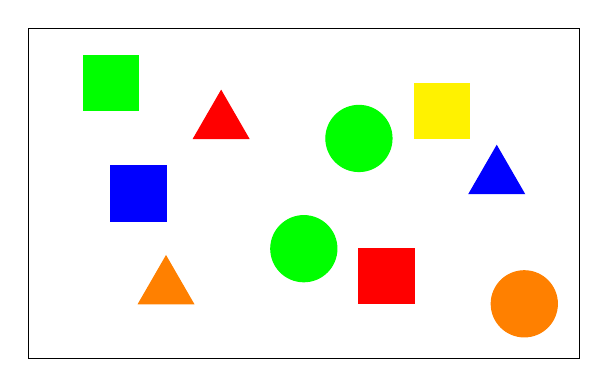
\begin{tikzpicture}[scale=0.7]
        \draw (0,0) rectangle (10,6);
        \filldraw[red] (3,4) -- +({cos(60)},{sin(60)}) -- +(1,0) -- cycle;
        \filldraw[orange] (2,1) -- +({cos(60)},{sin(60)}) -- +(1,0) -- cycle;
        \filldraw[blue] (8,3) -- +({cos(60)},{sin(60)}) -- +(1,0) -- cycle;
        \filldraw[green] (1,4.5) rectangle +(1,1);
        \filldraw[red] (6,1) rectangle +(1,1);
        \filldraw[yellow] (7,4) rectangle +(1,1);
        \filldraw[blue] (1.5,2.5) rectangle +(1,1);
        \filldraw[green] (5,2) circle (0.6);
        \filldraw[green] (6,4) circle (0.6);
        \filldraw[orange] (9,1) circle (0.6);
    \end{tikzpicture}
\end{center}

\begin{enumerate}
    \item Si l'on s'intéresse uniquement à la couleur des figures, quelles sont les issues ?
    \item Citer toutes les issues constituant les évènements suivants :
    \begin{enumerate}
        \item{Évènement R : << La figure est rouge >>}
        \item{Évènement C : << La figure est un carré >>}
    \end{enumerate}
    \item Les évènements ci-dessous sont-ils certains ? impossibles ?
    \begin{enumerate}
        \item{Évènement G : << La figure est une forme géométrique >>}
        \item{Évènement N : << La figure est de couleur noire >>}
        \item{Évènement D : << La figure est un disque >>}
    \end{enumerate}
\end{enumerate}